\documentclass{article}

\usepackage[T1]{fontenc}
\usepackage[czech]{babel}
\usepackage[utf8]{inputenc}
\usepackage{graphicx}

\graphicspath{ {imgs/} }

\def\code#1{\texttt{#1}}

\title{Vizualizace grafových algoritmů}
\author{Jakub Arnold}
\date{}

\begin{document}
\maketitle

Tématem práce je vizualizace grafových algoritmů, konkrétně prohledávání
do hloubky, do šířky, Dijkstrův algoritmus, hledání Eulerovské kružnice (nakreslení grafu jedním tahem)
v neorientovaných grafech, a Jarníkův algoritmus.

Všechny algoritmy jsou krokovatelné uživatelem, který zadá libovolný
graf (viz dále), a poté může krok po kroku sledovat, jak algoritmus
probíhá, a případně ho může pustit znovu z jiného počátečního vrcholu.

\section{Kompilace a spuštění}

Pro kompilaci je potřeba překladač, který umí C++11 (testováno na GCC 5.x, Clang 3.6, MSVC 14).
Dále je potřeba Qt5 (Qt4 nestačí), ale na konkrétní minor verzi by nemělo záležet.

Kompilace a spuštění se pak provede následovně:

\begin{itemize}
  \item \code{\$ qmake .}
  \item \code{\$ make}
  \item \code{\$ ./build/debug/graphite}
\end{itemize}

Testováno na různých distribucích Linuxu, včetně labu, OS X a zlehka na Windows.

\pagebreak

\section{Základní ovládání}

Program se ovládá klávesnicí i myší, kde všechny příkazy jdou zadat buď
přes hlavní menu a nebo pomocí klávesových zkratek.

\begin{center}
    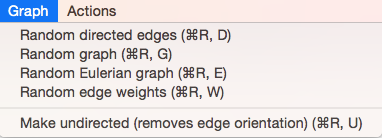
\includegraphics[width=0.5\textwidth]{KJaB5S6.png}
\end{center}

Zde je úplný seznam klávesových zkratek:

\begin{itemize}
  \item Vygenerování náhodného grafu \code{Ctrl-R G}.
  \item Náhodná oritentace hran \code{Ctrl-R D}.
  \item Vygenerování náhodného Eulerovského grafu \code{Ctrl-R E}.
  \item Náhodné ohodnocení hran \code{Ctrl-R W}.
  \item Odstranění orientace hran \code{Ctrl-R U}.
  \item Přidání vrcholu \code{A}.
  \item Spojení dvou vrcholů hranou \code{C}. Je potřeba napřed vybrat první, zmáčknout \code{C}, vybrat druhý, a zmáčknout \code{C} znovu.
  \item Smazání vrcholu nebo hrany \code{D}. (nejprve je potřeba hranu nebo vrchol vybrat kliknutím myši.)
  \item Označení počátečního vrcholu \code{S}.
  \item Start/Restart algoritmu \code{R}.
  \item Krok algoritmu \code{N}.
  \item Změna orientace hrany \code{O} (nejprve je potřeba hranu vybrat kliknutím myši.)
  \item Nastavení ohodnocení hrany \code{1-9}, nejprve je ale potřeba mít vybraný Dijkstrův algoritmus, jinak se ohodnocení hran nezobrazí, a poté kliknout na vybrané ohodnocení (*ne na hranu*).
\end{itemize}

Grafy je také možné uložit do souboru \code{Ctrl-S} a znovu načíst \code{Ctrl-O},
přičemž se zachová i rozložení vrcholů v prostoru (pokud je uživatel
přesunul.)

\pagebreak

\section{Používání programu}

Nejjednodušší je vybrat jeden z přiložených grafů v souboru, a otevřít
jej přes \code{File -> Open}, např. kompletní graf na 5 vrcholech v souboru
\code{examples/k5.g}.

\begin{center}
	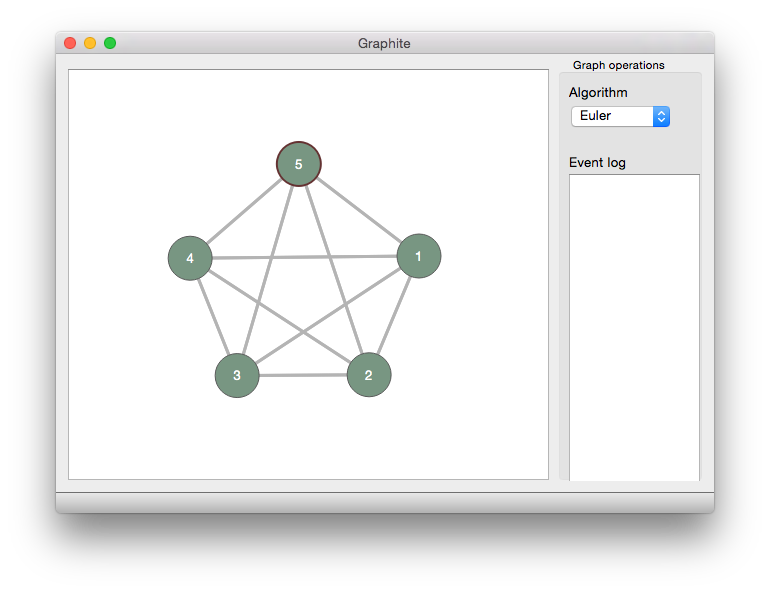
\includegraphics[width=0.8\textwidth]{iYrD1VK.png}	
\end{center}

V seznamu algoritmů vybrat Eulerovský tah.

\vspace{10pt}
\begin{center}
	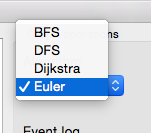
\includegraphics[width=0.25\textwidth]{ewrHxRO.png}
\end{center}
\vspace{10pt}

A kliknout na libovolný vrchol, vybrat ho jako počáteční (stisknutím \code{F}),
inicializovat algoritmus (stisknutím \code{R}), a poté již krokovat
stisknutím \code{N}. V libovolnou chvíli je možné znovu stiknout \code{R}, čímž se algoritmus
resetuje a začne pracovat odznova. \emph{Pokud uživatel graf jakkoliv změní
v průběhu algoritmu, je nutné algoritmus resetovat stisktnutím \code{R}}.

Většina důležitých informací které program provádí jsou vypisovány do
logu v pravé straně GUI (a některé navíc na STDOUT). Log v GUI je
editovatelný text, a lze ho tedy označit myší a smazat.

\pagebreak

\section{Generování náhodných grafů}

Aby bylo možné aplikaci jednoduše používat, obsahuje možnost
vygenerování náhodného souvislého grafu (žádný ze zabudovaných algoritmů
nedává smysl vizualizovat na nesouvislých grafech.) Graf je generován následujícím způsobem:

\begin{itemize}
  \item vygeneruje se 10-15 vrcholů, které se postupně spojí hranami, dohromady tvořící jednu velkou cestu
  \item každému vrcholu se s pravděpodobností 2/5 přidělí jedna další náhodná hrana
\end{itemize}

Takto vygenerovaný graf bude vždy souvislý, a díky malému počtu hran i
relativně přehledný. Graf je vždy generovaný jako neorientovaný. Pokud
si uživatel přeje, může poté náhodně zorientovat hrany (\code{Ctrl-R, D}).

\section{Generování Eulerovských grafů}

Protože pro Eulerovské grafy musí platit, že každý vrchol má sudý
stupeň, je také jednoduché nahlédnout, že musí ležet na nějaké kružnici.
Generování grafu tedy probíhá tak, že se nejprve vytvoří jednovrcholový
graf, a potom se 5-7krát vybere náhodný vrchol z grafu, a přilepí se na
něj další kružnice délky 3-5 (pro přehlednost.) Výsledný graf pak vypadá např. takto

\begin{figure}[!h]
  \centering
    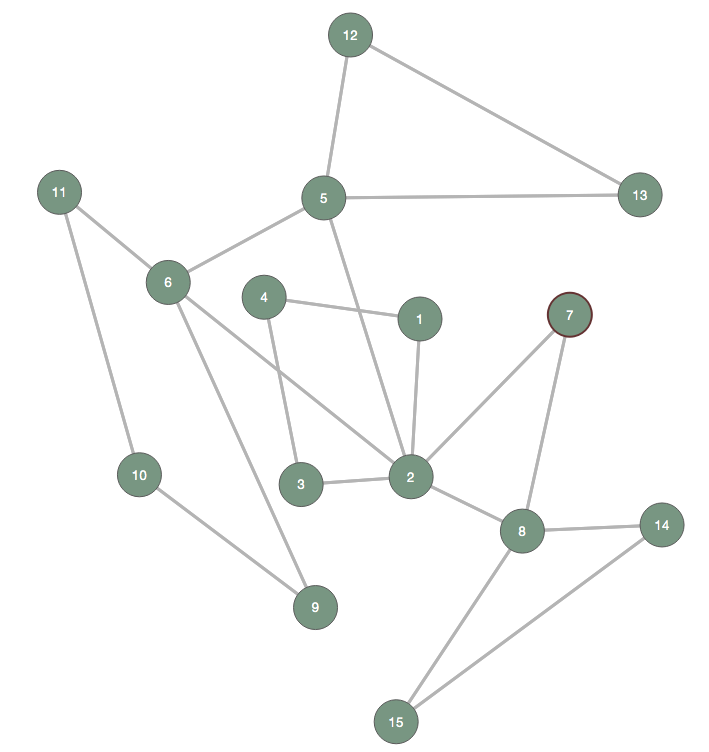
\includegraphics[width=0.5\textwidth]{LQNxfKa.png}
  \caption{Náhodný Eulerovský graf}
\end{figure}

Takto vygenerovaný graf má opět výhodu, že je díky menšímu počtu hran přehledný.

\subsection{Rozmístění vrcholů}

Při generování náhodného grafu jsou vrcholy vždy rozmístěny na spirálu,
která se rozvijí \emph{zevnitř ven}. Pro grafy výše zmíněné náhodně
generované grafy je toto rozložení relativně blízko tomu, co by si
uživatel mohl předstatovat, a stačí zpravidla pouze přemístit pár
vrcholů uvnitř spirály, aby se příliš mnoho hran nekřížilo.

\section{Algoritmy}

Všechny algoritmy jsou implementované jako stavový automat, ktery se
stiskem \code{R} přesune do počátečního stavu, a stiskem \code{N} postupně
krokuje, až dojde do koncového stavu, kdy algoritmus doběhl. Proto jsem zvolil
zásobníkovou variantu DFS místo rekurzivní, aby šlo jednoduše ovládat průběh algoritmu.

Všechny algoritmy pracují pouze na souvislých grafech. Pokud je graf nesouvislý,
algoritmus proběhne pouze na komponentě souvislosti ve které leží počáteční vrchol.
Toto řešení jsem zvolil převážně proto, že umožnuje uživateli větší graf rozpojit a sledovat
průběh pouze na části grafu, aniž by ho musel celý smazat a pak znovu vytvářet.

\subsection{DFS, BFS}

Pro porovnání prohledávání do hloubky a do šířky je nejlepší zvolit
stejný graf, a na něm pozorovat, jak se průběh jednotlivých algoritmů
liší. Oba používají stejnou konvenci, a to že nenavštívený vrchol je
tmavě zelený, otevřený je světle zelený a uzavřený je černý.

\begin{figure}[!h]
  \centering
    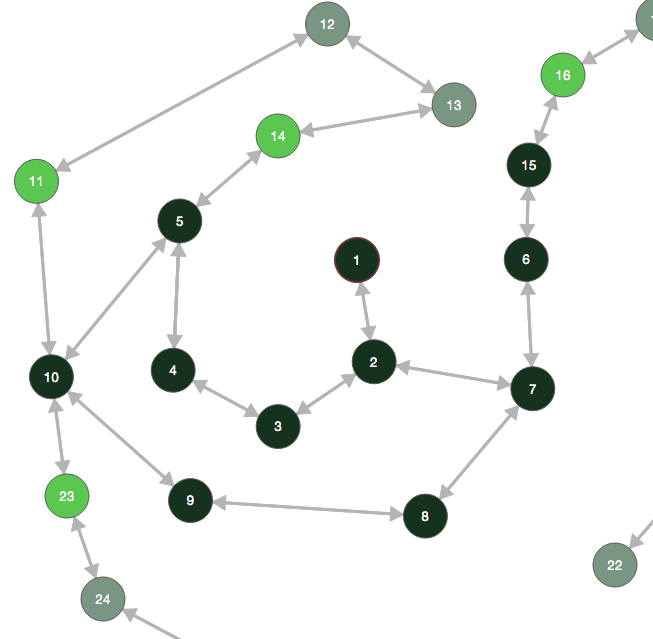
\includegraphics[width=0.5\textwidth]{CaAOrcu.png}
  \caption{Barvy vrcholů}
\end{figure}

Jak DFS tak BFS umí pracovat s orientovanými grafy. Orientace hrany se
změní označením hrany myší a stiskem \code{O}. Pro vrcholy \code{A} a \code{B} se
postupně mění typ hrany na \code{A -> B}, \code{A <- B}, a \code{A <-> B}.

\subsection{Dijkstrův algoritmus}

Dijkstrův algoritmus opět funguje i na orientovaných grafech, pričemž
navíc zobrazuje i ohodnocení hran.

\begin{figure}[!h]
  \centering
    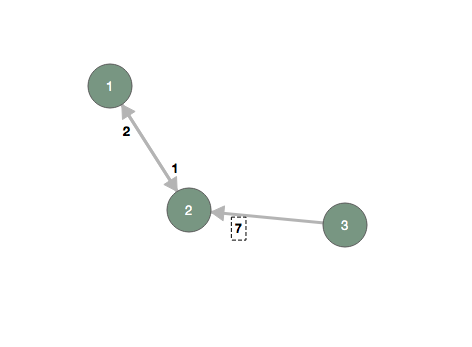
\includegraphics[width=0.5\textwidth]{2d7DzOA.png}
  \caption{Ohodnocení hran}
\end{figure}

Váha hrany je vždy zobrazena ve směru kam hrana ukazuje, a tedy pro
\emph{obousměrné}, resp. \emph{neorientované} hrany jsou zobrazena ohodnocení dvě,
každé jedním směrem.

Hranám lze nastavovat hodnoty v rozsahu 1-9, což se provede kliknutím na
ohodnocení hrany a stiskem patřičné klávesy 1-9. Označení se zobrazí
tečkovaným čtvercem okolo ohodnocení hrany (viz. obrázek).

Samotný dijkstruv algoritmus se poté zobrazuje podobně jako u DFS/BFS.
Nenavštívené vrcholy jsou tmavě zelené, otevřené jsou světle zelené a
uzavřené jsou černé. Navíc se však u vrcholů zobrazuje jejich vzdálenost
od počátečního vrcholu, a to tak, že se v popisku vrcholu zobrazí \code{číslo
vrcholu / vzdálenost od zdroje}. Vrcholy zatím neobjevené mají
nekonečnou vzdálenost, reprezentováno stringem \code{inf}, viz obrázek.

\begin{figure}
  \centering
    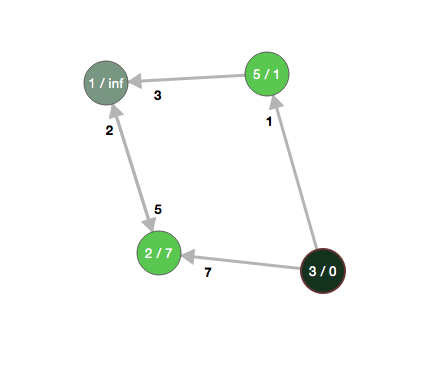
\includegraphics[width=0.5\textwidth]{OWYHOQ7.png}
  \caption{Průběh Dijkstrova algoritmu}
\end{figure}

\subsection{Eulerovská kružnice}

Algoritmus pro hledání Eulerovské kružnice se trochu liší od prvních
tří, a to tím, že funguje pouze na neorientovaných grafech, kde stupeň
všech vrcholů je sudý. Pokud je spuštěn na grafu který není Eulerovský,
nemusí správně fungovat.

Pro implemntaci jsem zvolil Fleuryho algoritmus, který funguje následovně:

\begin{enumerate}
  \item začni v libovolném vrcholu
  \item vyber hranu která není most, pokud jsou všechny mosty tak vyber libovolnou
  \item označ hranu jako smazanou, a přesuň se do vrcholu kam hrana ukazuje a opakuj krok 1.
\end{enumerate}

Tento algoritmus je velmi přímočarý, a ze všech implementací které jsem
zkoušel vede na nejnázornější vizualizaci, a to proto, že během svého
průběhu může označovat hrany které jsou mosty, a uživatel tak snadno
vidí, jak se algoritmus rozhoduje kudy půjde.

Na začátku algoritmu sice žádné mosty nemohou existovat, ale už po
prvním kroku dojde ke \emph{smazání} jedné hrany, a tím mohou nějaké mosty
vzniknout. Viz obrázek

\begin{center}
    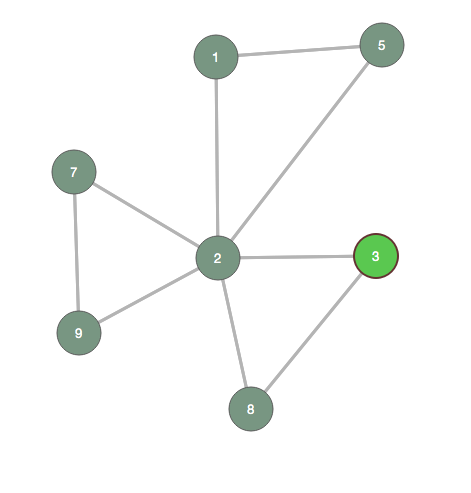
\includegraphics[width=0.5\textwidth]{95ubo0l.png}
\end{center}
\vspace{10pt}

a po prvním kroku už máme nalezeny dva mosty.

\vspace{10pt}
\begin{center}
    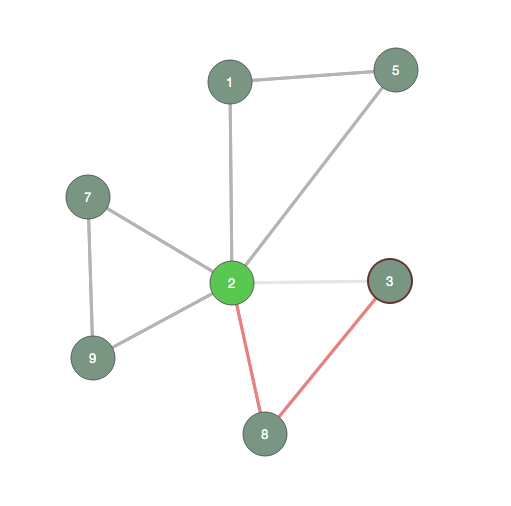
\includegraphics[width=0.5\textwidth]{Ls741t3.png}
\end{center}
\vspace{10pt}

Hledání mostů je nutné provést po každém kroku algoritmu, a probíhá
pomocí DFS klasifikace, konkrétně tak, že se prohledá celý graf pomocí
DFS, najdou se vrcholy, které leží na nějaké kružnici (pomocí zpětných
hran v DFS stromu), a ty co neleží jsou označený jako mosty.

Složitost algoritmu je tedy kvadratická, protože pro každý krok je nutné
provést celé DFS na odhalení mostů. Existují sice alternativní
algoritmy, které jsou ve výsledku rychlejší, ale z hlediska vizualizace mi přišel
Fleuryho algoritmus nejlepší.

\pagebreak

\subsection{Jarníkův algoritmus}

Poslední algoritmus který program implementuje je Jarníkův-Primův algoritmus
pro hledání nejlehčí kostry neorientovaného grafu. Při spuštění algoritmus automaticky
odstraní orientace všech hran, a není tedy nutné graf nijak dopředu opravovat.

Algoritmus lze spustit z libovolného vrcholu a vždy by se měl dobrat správného cíle,
a to najít nejlehčí kostru.

\begin{figure}[!h]
	\centering
	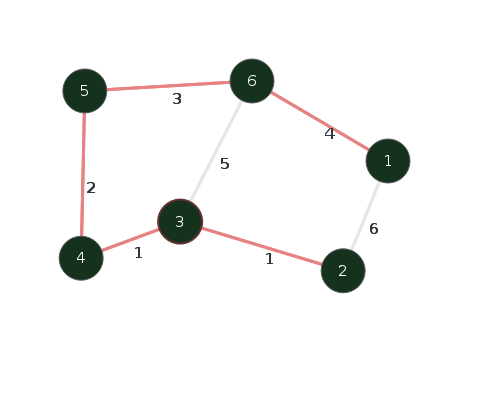
\includegraphics[width=0.7\textwidth]{kostra.png}
	\caption{Nalezená nejlehčí kostra}
\end{figure}

Samotná kostra je poté zobrazena červeně, a hrany které v kostře neleží jsou šedivé. Během průběhu
algoritmu jsou otevřené vrcholy obarveny světle zelenou, a uzavřené vrcholy černé.

\end{document}
